\documentclass{article}
\usepackage{amsmath}
\usepackage{tikz}
\usetikzlibrary{shapes, arrows.meta,arrows}
\tikzset{>=latex}
\usepackage[colorlinks=true, allcolors=blue]{hyperref}
\usepackage{pgfplots}
\pgfplotsset{compat=1.17}
\usepgfplotslibrary{fillbetween}

\begin{document}

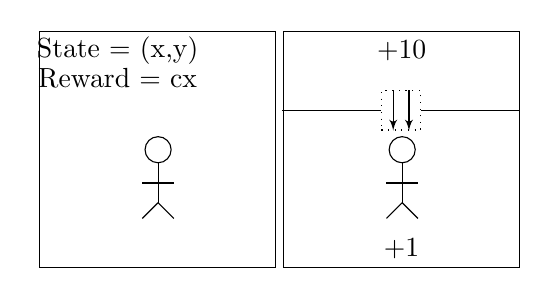
\begin{tikzpicture}[auto, node distance=2cm,>=latex']
    % draw borders
    \node[rectangle,fill=none, draw, minimum width=3cm, minimum height = 3cm] at (0.0, 0) (r_env) {}; 
    \node[rectangle,fill=none, draw, minimum width=3cm, minimum height = 3cm] at (3.1, 0) (t_env) {}; 

    % draw stickman in reward env
    \node[circle, fill=none, draw] at ([xshift=-1.5cm, yshift=+0.0cm]r_env.east) (head1) {};
    \draw (head1.south) -- ([yshift=-0.5cm]head1.south);
    \draw ([yshift=-0.5cm]head1.south) -- ([yshift=-0.7cm, xshift=-0.2cm]head1.south);  
    \draw ([yshift=-0.5cm]head1.south) -- ([yshift=-0.7cm, xshift=+0.2cm]head1.south);
    \draw ([yshift=-0.25cm, xshift=-0.2cm]head1.south) -- ([yshift=-0.25cm, xshift=+0.2cm]head1.south);

    % draw stickman in transition env
    \node[circle, fill=none, draw] at ([xshift=-1.5cm, yshift=+0.0cm]t_env.east) (head2) {};
    \draw (head2.south) -- ([yshift=-0.5cm]head2.south);
    \draw ([yshift=-0.5cm]head2.south) -- ([yshift=-0.7cm, xshift=-0.2cm]head2.south);  
    \draw ([yshift=-0.5cm]head2.south) -- ([yshift=-0.7cm, xshift=+0.2cm]head2.south);
    \draw ([yshift=-0.25cm, xshift=-0.2cm]head2.south) -- ([yshift=-0.25cm, xshift=+0.2cm]head2.south);

    % draw reward function in reward env
    \node at ([yshift=-0.25cm, xshift=1.0cm]r_env.north west) {{State = (x,y)}};
    \node at ([yshift=-0.6cm, xshift=1.0cm]r_env.north west) {{Reward = cx}};

    % add treadmil and walls
    \node[rectangle, dotted,fill=none, draw, minimum width=0.5cm, minimum height = 0.5cm] at ([yshift=+0.5cm, xshift=+1.5cm]t_env.west) (treadmill) {}; 
    \draw ([xshift=-1.25cm]treadmill.west) -- (treadmill.west);
    \draw ([xshift=1.25cm]treadmill.east) -- (treadmill.east);

    % add movement arrows
    \draw [->] ([xshift=-0.1cm]treadmill.north) -- ([xshift=-0.1cm]treadmill.south);
    \draw [->] ([xshift=0.1cm]treadmill.north) -- ([xshift=0.1cm]treadmill.south);

    % add goals
    \node at ([yshift=-0.25cm]t_env.north) {+10};
    \node at ([yshift=0.25cm]t_env.south) {+1};

\end{tikzpicture}

\end{document}